%%%%%%%%%%%%%%%%%%%%%%%%
%%% custom title page
%%%%%%%%%%%%%%%%%%%%%%%%%

% picture on title page
\usepackage{eso-pic}
\newcommand\BackgroundPic{
\put(0,0){%
\parbox[b][\paperheight]{\paperwidth}{
\vspace{0.5in}                          % adjust height of pic on page here
%\vfill
\centering
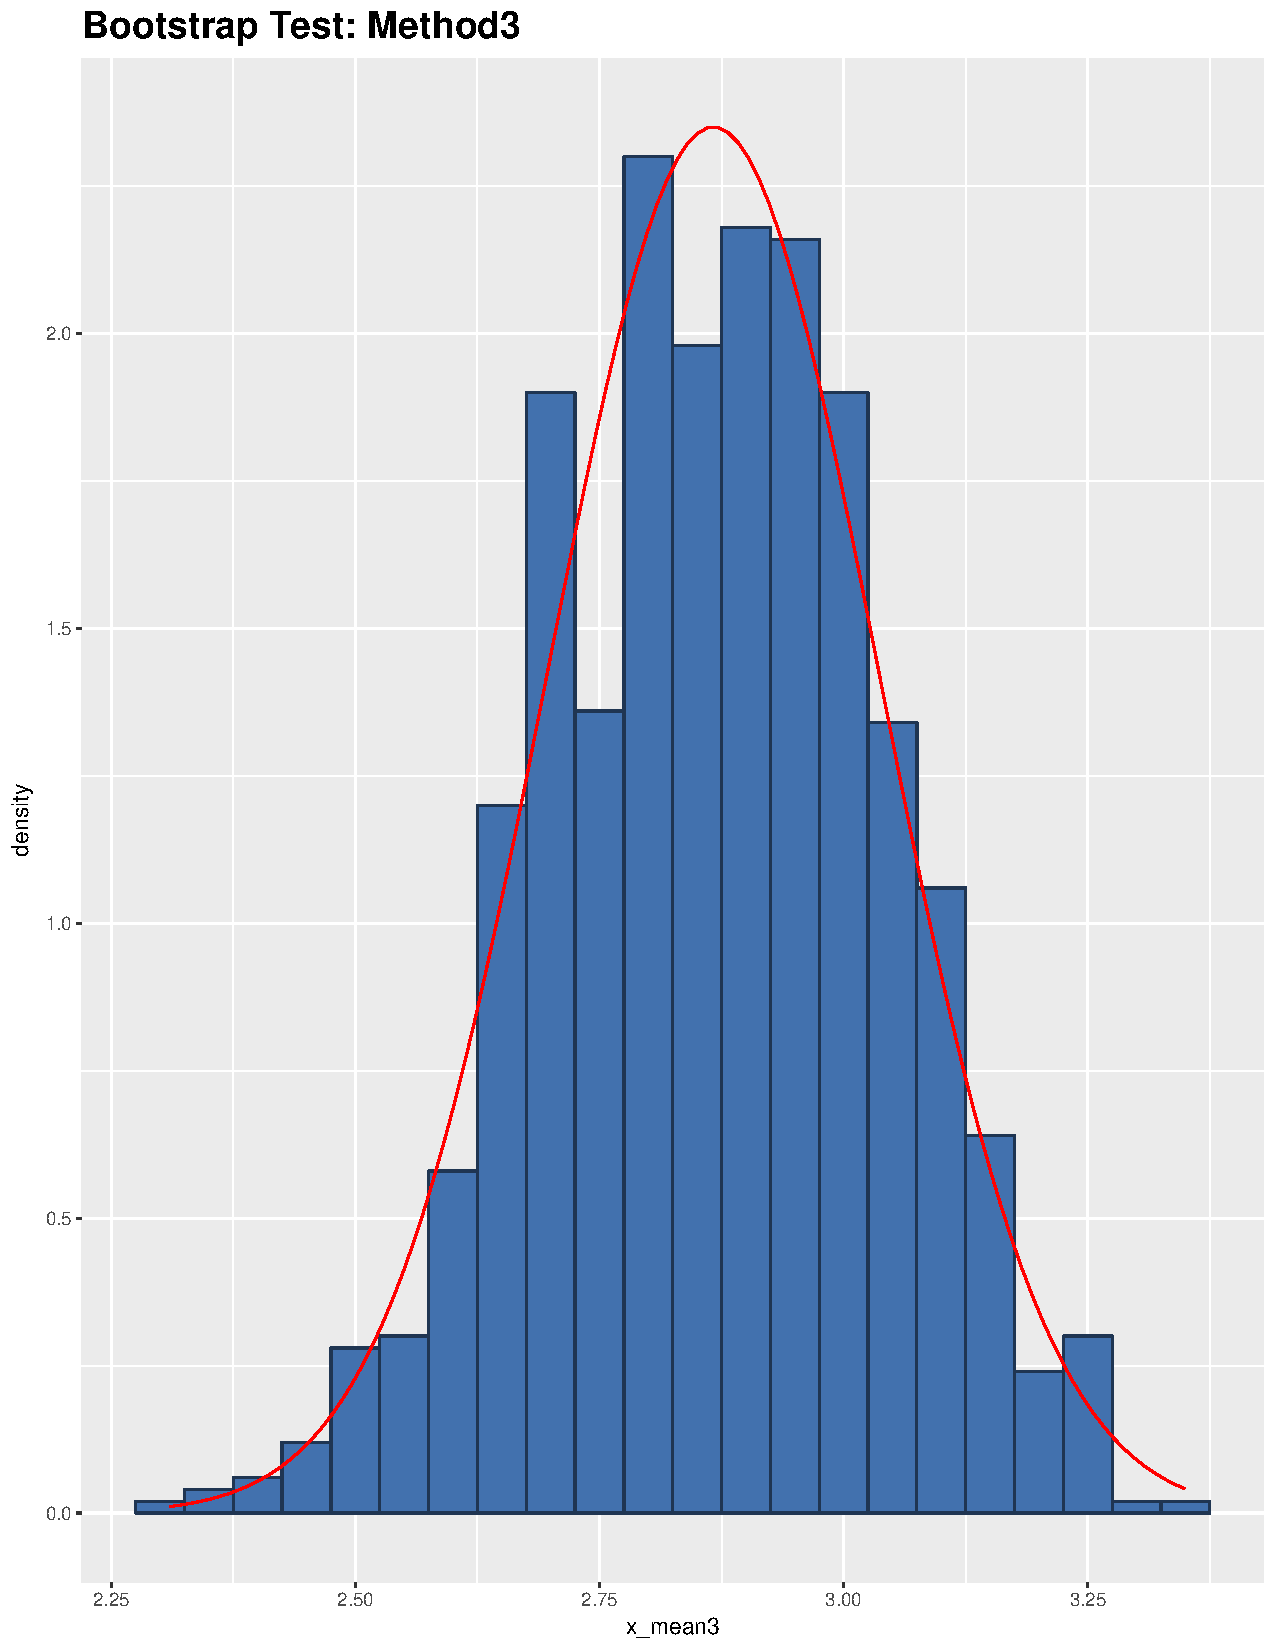
\includegraphics[width=6in, height=6in, keepaspectratio]{graphics/Rplot1}
%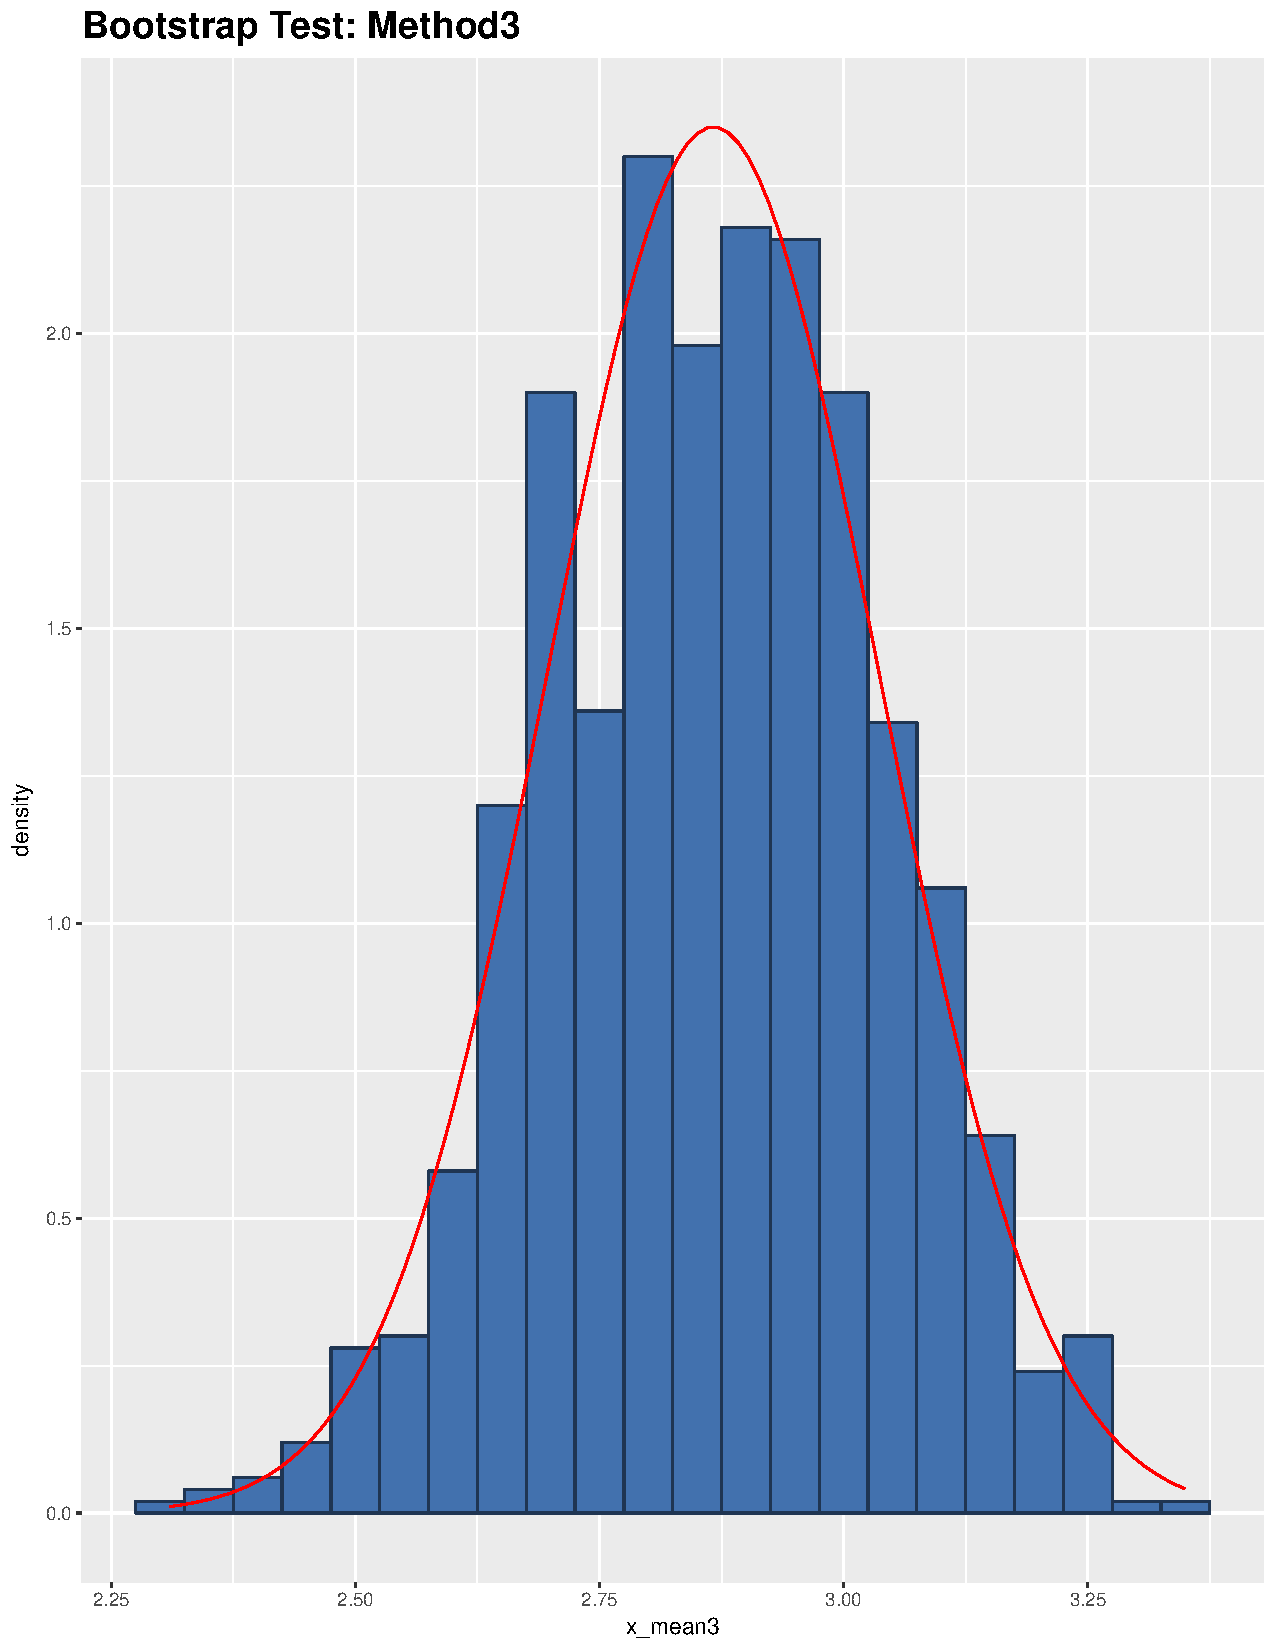
\includegraphics[width=\paperwidth, height=\paperheight, keepaspectratio]{graphics/Rplot1}
\vfill
}}}


% customize title page
\makeatletter                        % changes the catcode of @ to 11 to modify a package internal macro
\renewcommand{\maketitle}{
\thispagestyle{empty}
\AddToShipoutPicture*{\BackgroundPic}
\ClearShipoutPicture

% title
\phantom{}
\vspace{6in}                                    % adjust vertical here
%\vfill
\phantom{}
%\hspace{1in}
\hfill
\begin{tabular}[c]{@{}p{0.7\textwidth}@{}}        % adjust horizontal here
      \Large\@title\\
%      \Large\@author\\
%      \large\@date \\
%      \large{Portland, OR}\\

%      \color{white}\headingfont\LARGE\@title\\[1em]
%      \color{white}\headingfont\Large\@author\\[2em]
\end{tabular}


% client-author-date
\phantom{}
\vspace{0.25in}                  % adjust distance between tables here
%\vfill
\phantom{}
%\hspace{1in}
\hfill
\begin{tabular}[c]{@{}p{0.45\textwidth}@{}}
      \large{Produced for: ~ Film Profit, LLC}\\[0.25em]
      \large{Produced by: ~ \@author}\\
      %\@date \\


\end{tabular}

\clearpage
}
\makeatother                     % changes the catcode of @ back to 12
%%%


%%%%%%%%%%%%%%%%%
%%% fancy boxes
%%%%%%%%%%%%%%%%%
\usepackage{tcolorbox}
\usepackage{wrapfig}

\def\fullboxbegin{
\bigskip
\begin{tcolorbox}[colback=color1,colframe=color1,coltext=white,arc=0mm,boxrule=0pt]
}
\def\fullboxend{\end{tcolorbox}\medskip}
%


\def\leftboxbegin{
\begin{wrapfigure}{l}{0.5\textwidth}
\begin{tcolorbox}[colback=color1,colframe=color1,coltext=white,arc=0mm,boxrule=0pt]
}
\def\leftboxend{
\end{tcolorbox}
\end{wrapfigure}
}
%

\def\rightboxbegin{
\begin{wrapfigure}{r}{0.5\textwidth}
\begin{tcolorbox}[colback=color1,colframe=color1,coltext=white,arc=0mm,boxrule=0pt]
}
\def\rightboxend{
\end{tcolorbox}
\end{wrapfigure}
}

% counter
\newcounter{frames}
\def\frameboxbegin#1{
\bigskip
\refstepcounter{frames}
\begin{tcolorbox}[colback=white,colframe=color1,arc=0mm,title={\MakeUppercase{\textbf{Frame \arabic{frames}}: #1}}]
}
\def\frameboxend{
\end{tcolorbox}
}
%%%
